\begin{frame}
  \frametitle{Good Classical LDPC Code.}
  Example, the parity code on the Peterson graph.
  \begin{center}
  \scalebox{0.65} {
\begin{tikzpicture}

\Vertex[style={minimum size=0.01cm,shape=circle},NoLabel,x=3.5cm,y=7.0cm]{v0}
\Vertex[style={minimum size=0.01cm,shape=circle},NoLabel,x=0.0cm,y=4.3262cm]{v1}
\Vertex[style={minimum size=0.01cm,shape=circle},NoLabel,x=1.3369cm,y=0.0cm]{v2}
\Vertex[style={minimum size=0.01cm,shape=circle},NoLabel,x=5.6631cm,y=0.0cm]{v3}
\Vertex[style={minimum size=0.01cm,shape=circle},NoLabel,x=7.0cm,y=4.3262cm]{v4}
\Vertex[style={minimum size=0.01cm,shape=circle},NoLabel,x=3.5cm,y=5.0652cm]{v5}
\Vertex[style={minimum size=0.01cm,shape=circle},NoLabel,x=1.75cm,y=3.7284cm]{v6}
\Vertex[style={minimum size=0.01cm,shape=circle},NoLabel,x=2.4184cm,y=1.5652cm]{v7}
\Vertex[style={minimum size=0.01cm,shape=circle},NoLabel,x=4.5816cm,y=1.5652cm]{v8}
\Vertex[style={minimum size=0.01cm,shape=circle},NoLabel,x=5.25cm,y=3.7284cm]{v9}
%
\Edge[lw=0.005cm,labelstyle={pos=0.5},label=\hbox{$0$},](v0)(v1)
\Edge[lw=0.005cm,labelstyle={pos=0.5},label=\hbox{$1$},](v0)(v4)
\Edge[lw=0.005cm,labelstyle={pos=0.5},label=\hbox{$1$},](v0)(v5)
\Edge[lw=0.005cm,labelstyle={pos=0.5},label=\hbox{$0$},](v1)(v2)
\Edge[lw=0.005cm,labelstyle={pos=0.5},label=\hbox{$0$},](v1)(v6)
\Edge[lw=0.005cm,labelstyle={pos=0.5},label=\hbox{$1$},](v2)(v3)
\Edge[lw=0.005cm,labelstyle={pos=0.5},label=\hbox{$1$},](v2)(v7)
\Edge[lw=0.005cm,labelstyle={pos=0.5},label=\hbox{$0$},](v3)(v4)
\Edge[lw=0.005cm,labelstyle={pos=0.5},label=\hbox{$1$},](v3)(v8)
\Edge[lw=0.005cm,labelstyle={pos=0.5},label=\hbox{$1$},](v4)(v9)
\Edge[lw=0.005cm,labelstyle={pos=0.5},label=\hbox{$0$},](v5)(v7)
\Edge[lw=0.005cm,labelstyle={pos=0.5},label=\hbox{$1$},](v5)(v8)
\Edge[lw=0.005cm,labelstyle={pos=0.5},label=\hbox{$0$},](v6)(v8)
\Edge[lw=0.005cm,labelstyle={pos=0.5},label=\hbox{$0$},](v6)(v9)
\Edge[lw=0.005cm,labelstyle={pos=0.5},label=\hbox{$1$},](v7)(v9)
%
\end{tikzpicture} \ \ \ \begin{tikzpicture}
\Vertex[style={minimum size=0.01cm,shape=circle},NoLabel,x=3.5cm,y=7.0cm]{v0}
\Vertex[style={minimum size=0.01cm,shape=circle},NoLabel,x=0.0cm,y=4.3262cm]{v1}
\Vertex[style={minimum size=0.01cm,shape=circle},NoLabel,x=1.3369cm,y=0.0cm]{v2}
\Vertex[style={minimum size=0.01cm,shape=circle},NoLabel,x=5.6631cm,y=0.0cm]{v3}
\Vertex[style={minimum size=0.01cm,shape=circle},NoLabel,x=7.0cm,y=4.3262cm]{v4}
\Vertex[style={minimum size=0.01cm,shape=circle},NoLabel,x=3.5cm,y=5.0652cm]{v5}
\Vertex[style={minimum size=0.01cm,shape=circle},NoLabel,x=1.75cm,y=3.7284cm]{v6}
\Vertex[style={minimum size=0.01cm,shape=circle},NoLabel,x=2.4184cm,y=1.5652cm]{v7}
\Vertex[style={minimum size=0.01cm,shape=circle},NoLabel,x=4.5816cm,y=1.5652cm]{v8}
\Vertex[style={minimum size=0.01cm,shape=circle},NoLabel,x=5.25cm,y=3.7284cm]{v9}
%
\Edge[lw=0.005cm,labelstyle={pos=0.5,},label=\hbox{$0$},](v0)(v1)
\Edge[lw=0.005cm,labelstyle={pos=0.5,},label=\hbox{$0$},](v0)(v4)
\Edge[lw=0.005cm,labelstyle={pos=0.5,},label=\hbox{$0$},](v0)(v5)
\Edge[lw=0.005cm,labelstyle={pos=0.5,},label=\hbox{$1$},](v1)(v2)
\Edge[lw=0.005cm,labelstyle={pos=0.5,},label=\hbox{$1$},](v1)(v6)
\Edge[lw=0.005cm,labelstyle={pos=0.5,},label=\hbox{$0$},](v2)(v3)
\Edge[lw=0.005cm,labelstyle={pos=0.5,},label=\hbox{$1$},](v2)(v7)
\Edge[lw=0.005cm,labelstyle={pos=0.5,},label=\hbox{$1$},](v3)(v4)
\Edge[lw=0.005cm,labelstyle={pos=0.5,},label=\hbox{$1$},](v3)(v8)
\Edge[lw=0.005cm,labelstyle={pos=0.5,},label=\hbox{$1$},](v4)(v9)
\Edge[lw=0.005cm,labelstyle={pos=0.5,},label=\hbox{$0$},](v5)(v7)
\Edge[lw=0.005cm,labelstyle={pos=0.5,},label=\hbox{$0$},](v5)(v8)
\Edge[lw=0.005cm,labelstyle={pos=0.5,},label=\hbox{$1$},](v6)(v8)
\Edge[lw=0.005cm,labelstyle={pos=0.5,},label=\hbox{$0$},](v6)(v9)
\Edge[lw=0.005cm,labelstyle={pos=0.5,},label=\hbox{$1$},](v7)(v9)
%
\end{tikzpicture} 

}
\end{center}
\end{frame}

\begin{frame}
  \frametitle{Good Classical LDPC Code.} 
  
    Another example, the repttion code can be thought as the tanner graph defind by the parity code on the cyle graph.
    \begin{columns}[t]
      \begin{column}{0.4\textwidth}
    \begin{center}
      \scalebox{0.6}{
      \begin{tikzpicture}[scale=1]
      \draw
        (8.0, 0.0) node[shape=circle,draw=black] (0){}
        (7.825, 0.624) node[shape=circle,draw=black] (1){}
        (7.308, 1.22) node[shape=circle,draw=black] (2){}
        (6.472, 1.763) node[shape=circle,draw=black] (3){}
        (5.353, 2.229) node[shape=circle,draw=black] (4){}
        (4.0, 2.598) node[shape=circle,draw=black] (5){}
        (2.472, 2.853) node[shape=circle,draw=black] (6){}
        (0.836, 2.984) node[shape=circle,draw=black] (7){}
        (-0.836, 2.984) node[shape=circle,draw=black] (8){}
        (-2.472, 2.853) node[shape=circle,draw=black] (9){}
        (-4.0, 2.598) node[shape=circle,draw=black] (10){}
        (-5.353, 2.229) node[shape=circle,draw=black] (11){}
        (-6.472, 1.763) node[shape=circle,draw=black] (12){}
        (-7.308, 1.22) node[shape=circle,draw=black] (13){}
        (-7.825, 0.624) node[shape=circle,draw=black] (14){}
        (-8.0, 0.0) node[shape=circle,draw=black] (15){}
        (-7.825, -0.624) node[shape=circle,draw=black] (16){}
        (-7.308, -1.22) node[shape=circle,draw=black] (17){}
        (-6.472, -1.763) node[shape=circle,draw=black] (18){}
        (-5.353, -2.229) node[shape=circle,draw=black] (19){}
        (-4.0, -2.598) node[shape=circle,draw=black] (20){}
        (-2.472, -2.853) node[shape=circle,draw=black] (21){}
        (-0.836, -2.984) node[shape=circle,draw=black] (22){}
        (0.836, -2.984) node[shape=circle,draw=black] (23){}
        (2.472, -2.853) node[shape=circle,draw=black] (24){}
        (4.0, -2.598) node[shape=circle,draw=black] (25){}
        (5.353, -2.229) node[shape=circle,draw=black] (26){}
        (6.472, -1.763) node[shape=circle,draw=black] (27){}
        (7.308, -1.22) node[shape=circle,draw=black] (28){}
        (7.825, -0.624) node[shape=circle,draw=black] (29){};
      \begin{scope}[-,draw opacity=0.5]
        \draw (0) to node[] {$1$} (1);
        \draw (0) to node[] {$1$} (29);
        \draw (1) to node[] {$1$} (2);
        \draw (2) to node[] {$1$} (3);
        \draw (3) to node[] {$1$} (4);
        \draw (4) to node[] {$1$} (5);
        \draw (5) to node[] {$1$} (6);
        \draw (6) to node[] {$1$} (7);
        \draw (7) to node[] {$1$} (8);
        \draw (8) to node[] {$1$} (9);
        \draw (9) to node[] {$1$} (10);
        \draw (10) to node[] {$1$} (11);
        \draw (11) to node[] {$1$} (12);
        \draw (12) to node[] {$1$} (13);
        \draw (13) to node[] {$1$} (14);
        \draw (14) to node[] {$1$} (15);
        \draw (15) to node[] {$1$} (16);
        \draw (16) to node[] {$1$} (17);
        \draw (17) to node[] {$1$} (18);
        \draw (18) to node[] {$1$} (19);
        \draw (19) to node[] {$1$} (20);
        \draw (20) to node[] {$1$} (21);
        \draw (21) to node[] {$1$} (22);
        \draw (22) to node[] {$1$} (23);
        \draw (23) to node[] {$1$} (24);
        \draw (24) to node[] {$1$} (25);
        \draw (25) to node[] {$1$} (26);
        \draw (26) to node[] {$1$} (27);
        \draw (27) to node[] {$1$} (28);
        \draw (28) to node[] {$1$} (29);
      \end{scope}
    \end{tikzpicture}
 
  }
  \end{center}
\end{column}
\begin{column}{0.25\textwidth}
\begin{equation*}
    \begin{split}
     \overbrace{ 
      \begin{bmatrix}
        1 & 1
      \end{bmatrix}
    }^{ \text{ parity check matrix of } C_{0} }
    % \mathbb{F}_{2}^{1 \times 2} 
  \end{split}
\end{equation*}
\begin{center}

\begin{tikzpicture}
    \draw (0,0) circle (6pt);
    \draw[ - ]  (0,0) to (1,1); 
    \draw[ - ]  (0,0) to (1,-1); 
    %\uncover<2->{\node (D) at (-4,1) { $110101$ } ;  
  \end{tikzpicture}
\end{center}
\end{column}
\begin{column}{0.35\textwidth}
  \begin{equation*}
    \begin{split}
      \overbrace{ 
      \begin{bmatrix}
1 & 1 & 0 & 0 & 0 & 0 \\
0 & 1 & 1 & 0 & 0 & 0 \\
0 & 0 & 1 & 1 & 0 & 0 \\
0 & 0 & 0 & 1 & 1 & 0 \\ 
0 & 0 & 0 & 0 & 1 & 1 \\
1 & 0 & 0 & 0 & 0 & 1 
 \end{bmatrix}
 }^{  \substack{ \text{ Parity check matrix of } \mathcal{T} \left( \Gamma, C_{0} \right) \\ \text{  Each row associated with vertex check. }} }
    \end{split}
  \end{equation*}
\end{column}
\end{columns}
  \end{frame}


